\documentclass[../main/main.tex]{subfiles}

\newdate{date}{14}{05}{2020}

\begin{document}

\section{Lecture 20}
 \displaydate{date}.  Compiled:  \today. Martina 
 
\subsubsection{Slide 330}

\begin{figure}[h!]
\centering
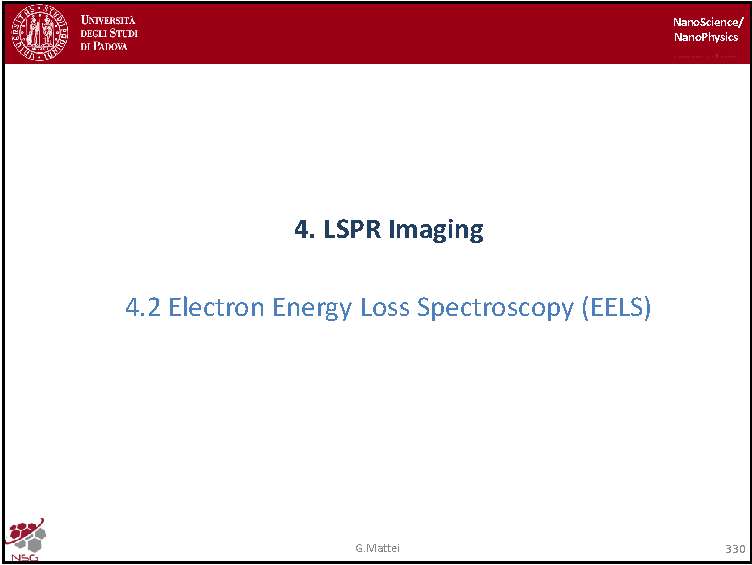
\includegraphics[page=1,width=0.9\textwidth]{../lessons/pdf_file/20_lesson.pdf}
\end{figure}

Another very effective technique for imaging the localized surface plasmon resonance in plasmonic systems is the Electron Energy Loss Spectroscopy or EELS. This technique is normally operated within transmission electron microscope and it is able to obtain very high spatial resolution down to below $1 nm$ in size, with a very high energy resolution so that you can obtain very accurate imaging of the resonance in the near field, it is in principle able to show more or less what you can do by simulation calculation in your system.

\newpage

\subsubsection{Slide 331}

\begin{figure}[h!]
\centering
\includegraphics[page=2,width=0.9\textwidth]{../lessons/pdf_file/20_lesson.pdf}
\end{figure}

Let's see how this technique works. Normally you send a point-like electronic beam with very high energy of the order of $100/300 keV$ which can be reduced in size down to something below $1 nm$ at a half maximum of the electron beam, so a very sharp point-like beam, which can be scanned or positioned very accurately close to the NP or at an arbitrary distance with respect to the NP center. 

So to simplify the description imagine to have spherical NP with dielectric function $\epsilon(\omega)$, the radius of the NP is $R$ and suppose that we are sending an electronic beam at a distance $=d$ perpendicular to the trajectory of the electrons, which travel at a velocity $=v$; we can describe the electron trajectory in semi-classical approximation as a $=r(t)==d+=vt$ where at $t=0$ the electron is exactly at distance $=d$ from the NP. 

Of course when the electron or each electron is passing in this direction with respect to the NP, if there are free electrons or polarizable electrons in our system they will feel the incoming electrons, so that they will be repelled and they will move far from the electronic beam, but as soon as the electron is passed, they will back to the original position, from the restoring force, so that there is an induced electric dipole which induces an electric field, so that this induced electric field is able to interact with incoming electrons in the beam, so that you can easily calculate what is the energy lost by the electrons passing at this distance with respect to the NP to induce the oscillation of the plasmon in the NP and this is easily calculated by calculating the force exerted by the induced field on the electrons which is nothing but the induced field times the electronic charge.

Of course the induced field is a function of the coordinate and of time and if we multiply or if we project this force on the trajectory, this is nothing but the work, so if we integrate in time, this is the energy loss of the electrons passing through this trajectory here, due to the interaction with the induced field on the NP.

Of course we can recast this time integral into a frequency integral by working with a Fourier transform of the integrand function, this function is called the Loss Probability and it can be written this way here, so that we can obtain a spectral information, the spectral dependency of the Loss Probability for the electrons, because this will give us chance to obtain the resonant behaviour when the frequency matches the resonant frequency or the modal frequency of the oscillation of the charge in the NP.

So with this simple qualitative description of the basic physics going on in the system you can clearly understand that with this technique it will be easy to obtain an excitation from one site of the modes of oscillation and as we will see even of those modes which are dark modes, which cannot be excited by photons, due to the geometry of the plane wave excitation with photons.

\newpage

\subsubsection{Slide 332}

\begin{figure}[h!]
\centering
\includegraphics[page=3,width=0.9\textwidth]{../lessons/pdf_file/20_lesson.pdf}
\end{figure}

So, let's see the effect of this EELS technique on the characterization of the local field around NP. The main result can be seen in this image here, which is extracted from this beautiful paper. The experiment was like that, with a transmission electron microscope operated in scanning transmission electron microscope, that is a mode in which the beam can be made point-like, so very sharp, with a full width at half maximum of around $1 nm$ in size. 

The beam can be rastered over the particle, in this case the contrast in this image is triggered by the scattering produced by the crystalline structure or the atomic structure in the system, so that we have dark background and a bright contrast on the NP because the background is made out of carbon and the NP in this case is silver, so very high atomic number, so the scattering as in the Rutherford cross-section produces very large scattering so that the bright contrast here is indication.

But for our purposes what is interesting is that if we scan along this line and we take point by point the EELS spectrum in which we have here the energy or the frequency and here the intensity which is the number of electrons which suffered that specific energy loss in the system, we see that the specific losses are reported here as a function of the position. 

Suppose we are here that is outside or at the surface or close to the surface of our NP, and we have this very intense peak here in the EELS spectrum at around $3.3 eV$, and as soon as we move more and more within the inside of the NP, we obtain the excitation additional peak at slightly higher energy, that is $3.8 eV$ and you can clearly see here when you are exactly in the middle this will have the maximum of intensity and at the same time the previous peak decreases in intensity, so there is a transfer of energy between this two modes, when the beam is outside or is inside the NP. 

Of course the situation is symmetric when you go on the other direction here and you reach the external position in which basically you will recover the original spectrum at the single peak of $3.3 eV$.

So, what is the physical interpretation of this result? The interpretation which can be obtained by modelling the structure of our nanosystem is that the peak at $3.3 eV$ is nothing but the surface plasmon resonance excited by the Coulomb interaction or repulsion between the incoming electron beam and the free electrons in the particle, if you convert $3.3 eV$ in wavelength it is nothing but $380 nm$ so exactly what is expected for a silver NP, the diameter is around $25 nm$ in this case, and so that is exactly what is expected for silver NP in vacuum in this case, we are i the ultra high vacuum, so that the Fr\"olich condition is fulfilled at lower wavelengths with respect to that of silica.

In this particular case the true structure of our system is silver NP surrounded by tiny layer of citrate, which is a passivating agent which is a bioproduct of the synthesis and by the way this will be the synthesis that we will see in the lab activity for our purposes.

The first peak is as I mentioned the localized surface plasmon resonance of the structure, which of course is of high intensity when the beam is outside that the dipolar mode can be easily excited. Of course when we are entering in the bulk of the particles we will see this additional peak at higher energy, which means lower wavelength ($32o nm$), and this is nothing but the bulk plasmon resonance of silver, you may remember that in the solid state physics course you where taught that the bulk plasmon resonance cannot be excited by photons, but historically they were discovered exactly by shining an electronic beam on a thin foil of the metal, and in this case you have exactly the very same effect and this energy exactly matches the bulk plasmon frequency for silver. 

\newpage

\subsubsection{Slide 334}

\begin{figure}[h!]
\centering
\includegraphics[page=4,width=0.9\textwidth]{../lessons/pdf_file/20_lesson.pdf}
\end{figure}

It is very interesting to use this EELS technique to obtain information which can be size-dependent; in this experiment silver NP with dfferent sizes ranging from $11 nm$ down to $1.7 nm$ in radius were measured with the EELS by exciting the system outside or in close proximity to the surface, so that just the surface plasmon resonance was excited and people were able to spot that position of the peak suffer a shift in energy with respect to the size, as you can see clearly in this picture here, that is at a larger is the particle, at the lower s the energy of the transition. 

This is an indication that there is a transition between the classical description toward the quantum description in which we need to modify the dielectric function basically to obtain the spectral position of our resonance as a function of the size, and this is beautiful demonstration that the procedure that we used for the correction with the s-electrons can be very effective.

If you report quantitatively the position in energy of the surface, the surface plasmon resonance, as a function of the diameter, you can clearly see that there is this behaviour here when the size is going down of course with certain error, but of course the trend is very clear, whereas if you point the electronic beam on the bulk of the NP, the position of the bulk plasmon frequency is almost independent of the size, so that is a clear indication that the two properties can be obtained with a model that we introduce phenomenologically for correcting the dielectric function.

\newpage

\subsubsection{Slide 335}

\begin{figure}[h!]
\centering
\includegraphics[page=5,width=0.9\textwidth]{../lessons/pdf_file/20_lesson.pdf}
\end{figure}

If you look at the analytic model you may remember that we described the dielectric function in terms of the Drude-Lorentz model introducing the oscillation in frequency of the bounded electrons and of the free electrons part which is the intraband part here of the dielectric function collected for this additional term here.

And with this analytic model it s possible to follow the evolution as a function of the diameter of the expected position of the resonance with respect to the size whereas for the bulk more or less a constant value is obtained as expected from the experiment, and there is also quantum mechanic calculation with density functional theory model which are able to obtain quantitative prediction for the very same fact and the results are very interesting because they match exactly the evolution of the experimental point. So this is a clear indication that the quantum confinement of the electrons can be seen directly here in the experiment.

\newpage

\subsubsection{Slide 336}

\begin{figure}[h!]
\centering
\includegraphics[page=6,width=0.9\textwidth]{../lessons/pdf_file/20_lesson.pdf}
\end{figure}

And another very interesting thing that you can do with EELS is the near field mapping, you are able not only to excite the modes but also to describe the spatial evolution of those modes.

Let's see for instance as in this experiment, let's change from spherical particles to rod-like particles like in this case, so we will have an asymmetric particles, the polarization in this case is very important, you may remember that if light goes in this direction and the electric field is polarized in this direction, you excite the transverse mode whereas the longitudinal modes can be excited by photons in this direction, and if you calculate the extinction cross-section you can easily obtain these two peaks as expected from the theory and of course this corresponds to different modes of oscillation of course, different energy or wavelengths in terms of the modes, and in this case we have the excitation in the longitudinal direction, whereas in the b configuration in which we have excitation along the transverse direction, of course electrons oscillate according to this.

Of course this two modes can be excited by photons but they can also be excited by electrons passing in close proximity to the NP, in particular if we go with the beam in this point here of course the repulsion of the electrons will go in this direction so we will excite the longitudinal modes and viceversa if we stay with the beam here we will excite the transverse mode, and by calculating the energy loss function in this case the loss probability is exactly what you ca expect for the measurements of the cross-section for photons, so this is an indication that the two quantities are strongly related, because they produce the very same spectral effect on the system.

Of course also in this case the position of the electronic beam with respect to the NP will produce different configuration of the electronic oscillation, but this is exactly consistent with the optical description. Moreover experimentally you can also map, that is if you scan the position of your beam all over the image point by point, so you can reconstruct the value of the energy loss, the intensity map point by point, so that you can assign to each pixel of this image a value of the energy loss function, and you can clearly see that in this case the local intensity of the loss function matches the one of the near field map in the system, of course for each position you can record the full spectrum in energy and then you can assign to each spectrum the resonances in terms of the modes of your oscillations, of course when the beam is positioned here or here the most intense resonance will be the transverse mode of the electronic beam.

So this is really a very exciting technique for mapping the near field with a very high spatial resolution, so this can be comparable to simulation. 

\newpage

\subsubsection{Slide 337}

\begin{figure}[h!]
\centering
\includegraphics[page=7,width=0.9\textwidth]{../lessons/pdf_file/20_lesson.pdf}
\end{figure}

But this is not the only thing that you can do with this technique, as reported in this paper here, people were able to excite even dark modes, you may remember that dark plasmons are configurations in which you have interacting NP in which there is an out of phase inducing dipole moments on the two neighbour particles, for instance in this case people used two nano-rods with this beam configuration, and of course, if you excite from this direction, you can excite the modes in this direction here, if you enter with the beam on this side and you polarize the electric field in this direction, you will excite different modes.

The idea here is that of course configuration c can be excited because you have in phase dipole moments induced on the two rods. On the contrary the d configuration is a dark plasmon because the two dipoles are out of phase of $\pi$ so they cannot be excited by optical modes, whereas the modes in e are bright modes, so they can be excited by photons.

Of course you can also obtain the same effect by exciting the system with electrons, you can calculate the EELS probability map, and so again in this case you can clearly see that you can obtain exactly what is expected for our dark modes excited with electron beam, and experimentally you can obtain very nice agreement with the theory, and if you excite here you have this configuration with this structure in the spectrum c, but what is interesting is that when you excite here you can excite exactly the dark plasmon, which is the spectrum d, which is not possible with optical excitation and of course you can map the intensity of the plasmonic modes by looking point by point at the intensity map around the NP and you can clearly see what is the field distribution around the particles in all the three configurations.

So this is a clear proof that all the modes that you can calculate can be excited whit electrons, not by photons in real experiments, but of course they can be calculated on the basis of pure electrodynamic calculations as you can see in these simulations here.

\newpage

\subsubsection{Slide 338}

\begin{figure}[h!]
\centering
\includegraphics[page=8,width=0.9\textwidth]{../lessons/pdf_file/20_lesson.pdf}
\end{figure}

So as you have seen EELS is a very powerful technique to probe also the plasmonic behaviour at the nanoscale with this near field capabilities in terms of spatial resolution and the additional capability to excite even dark modes, which cannot be excited by photons. 

In this paper people investigated another complexly shaped NP which are silver nanoprisms with lateral size $L$ and thickness $t$ and they were able to measure different modes of oscillation of the electrons in the system, by taking maps of the intensity of the energy loss as a function of the position around and on top of the particle, and point by point they collected an energy loss spectrum that is the intensity versus the energy loss, and so they reconstructed energy by energy the local intensity of the loss, so by reconstructing this sort of hyper-spectral imaging mode, that is at each point is associated a spectrum, not a single point, so that you can read for different energies the modes of oscillation.

So when you are in $1.65 eV$ in energy you are more or less at this position here, and this position here is strongly excited in this configuration here. When you have the hotspots at the tips of the prism, which is clear expected mode when you have even optical excitation, of course at different energy like in this case $2.55 eV$ basically probe this mode here, and you can clearly see that this can be excited, the density is related in the midway in between the sharp points of the prisms, or at $3.50 eV$ you excite the higher energetic modes in our system, which is a close resemblance of the bulk mode in our system.

And of course you have different values of that because of the quantum confinement effect in our system, indeed if you change the thickness and the lateral size you can move and increase the intensity of those resonances and you practically see the very same modes that you already have seen for the smaller nanoprisms but now with a sharper intensity.

So actually as a final comment the EELS technique is really a powerful tool for investigating plasmonic properties with this very high spatial resolution and this is a clear proof that the level of agreement that you can obtain with optical simulation, electrodynamic simulation and real world experiments is really remarkable with the techniques that we described so far, and validated not only in the far field, because it is very straightforward to measure cross-sections, but in the near field it is very a quite demanding problem to obtain meaningful information on the field distribution.

Of course this is very important to obtain such information, not only for the fundamental characterization of our system or for the validation of the simulations, but it is also important to obtain functionalities out of your system, in particular, if you want to couple a nanostructure to an emitter to change its quantum efficiency you need to know where you have to put the emitter close to the nanostructure to have a near field coupling, to have chances to enhance the quantum efficiency of the emitter, and this will be the subject of the next chapter.

\newpage

\subsubsection{Slide 339}

\begin{figure}[h!]
\centering
\includegraphics[page=9,width=0.9\textwidth]{../lessons/pdf_file/20_lesson.pdf}
\end{figure}

The problem that I would like to discuss now is a very fundamental one and one of the most interesting in terms of the applications of nanophotonics nowadays and it is the coupling of suitable quantum emitter to nanostructures with engineered optical states so that we can obtain a very interesting phenomenon which is the modification of the quantum efficiency of the emitter in close proximity to the nanostructure. The problem of course is highly complex in terms of the physical description, but we will try to follow a very simple phenomenological approach. 

\newpage

\subsubsection{Slide 340}

\begin{figure}[h!]
\centering
\includegraphics[page=10,width=0.9\textwidth]{../lessons/pdf_file/20_lesson.pdf}
\end{figure}

We would like to describe for instance in particular the basic phenomenon which is why in principle we should expect a modification of the quantum efficiency of an emitter which is near field coupled to a nanostructure.

You may remember that spontaneous emission in a two level emitter can be described by this simple picture here. You have an excitation triggered by a photon, it will excite the atom or the quantum emitter from the ground state to the excited state and then the deexcitation of the system will produce the photon which is emitted. 

The initial state of the emission is zero photons and the emitter in the excited state; the final state will be described by the emitter in the ground state and one photon in some photonic state of the system, so this spontaneous emission can be influenced by the presence around the emitter of a suitably engineered optical density of states, if you are able to modify the states allowed for the photons, you can extract more easily the energy for that specific transition in your system. This is what I would like to briefly describe you in the next slides.

\newpage

\subsubsection{Slide 341}

\begin{figure}[h!]
\centering
\includegraphics[page=11,width=0.9\textwidth]{../lessons/pdf_file/20_lesson.pdf}
\end{figure}

To calculate what is the emission rate of a quantum emitter in a given optical environment, if we start from the unperturbed emitter eigenfunction, so if $\psi_i$ is the system without the presence of photons, the photon field will perturb the Hamiltonian of the emitter $H_0$ producing a new Hamiltonian $H=H_0+V$ which can be easily written as the scalar product between the electric field times the dipole operator of the transition, and so of course this perturbation provided that it is not too strong with respect to the energy of $H_0$ will produce a transition between levels, and you can obtain a transition from initial state to a final state provided that the energy conservation is satisfied. 

To obtain a quantitative description of this, the rate of decay of the initial state $\psi_i$ can be described by the Fermi's Golden Rule, which is nothing but the decay rate contribution which can be written as this well known formula here in which there are the probability between the initial and all the final allowed states so that you can rewrite also this expression making use of the density of states of the final states provided that you have all the possibilities to have access to those states, so you have the transition matrix, the square modulus of that, times the density of states, the higher is the density of states the higher is the decay rate of your system, so you can accelerate or enhance the decay rate if you are able to modify this density of optical states.

Of course when you are dealing with experimental systems what you measure is not exactly the only radiative transitions, but also the global the decay rate that is the radiative plus the non radiative contribution, and in general the non radiative contribution is due to recombination centers or phonon coupling or defects coupling, so this will not produce photons in the far field, but it's a way to affect also the decay rate globally, so the global probability is nothing but the sum of the probability of the two decay rates, that is the radiative and the non radiative one.

\newpage

\subsubsection{Slide 342}

\begin{figure}[h!]
\centering
\includegraphics[page=12,width=0.9\textwidth]{../lessons/pdf_file/20_lesson.pdf}
\end{figure}

One of the most exciting demonstration of this effect which can be unexpected, so how can we speed up or improve the efficiency of an emitter, was given in this beautiful paper by Drexhage, in which he studied the lifetime variation, and if you are able to control the relative distance between the emitter in this case sketched as a dipolar emitter, in this experiment the emitter were Europium3+ ions in close proximity to a silver mirror, that is an infinitely thick filled by silver, in which you could control the relative distance between the emitter and the silver mirror through a spacer done with a polymer with very controlled positioning system.

So Drexhage was able to measure variation in the lifetime as a function of the position, and he was able to measure this oscillating behaviour which can be nicely reproduced by a classical dipolar oscillator model which is nothing but a description in the Green function formalism of the field, the interaction between the emitter and the field induced in the mirror, so that the lifetime can be largely affected by the relative distance between emitter and the silver mirror because the emitter emits at a given wavelength, so that distances can be of relevance in our system. 

For instance Europium emits around $610 nm$ and the strong interaction came for distances much lower than this wavelength of course, because this is not a far field property but it is strictly a near field property like nicely sjetched here.

\newpage

\subsubsection{Slide 343}

\begin{figure}[h!]
\centering
\includegraphics[page=13,width=0.9\textwidth]{../lessons/pdf_file/20_lesson.pdf}
\end{figure}

The description of the physics of the system is a little bit complicated, I would like just to show you how to describe the coupling between a two level emitter sketched as a given dipole of coordinate $r_m$ at a given distance $z$ with respect to a spherical NP so the same effect was demonstrated by Drexhage for a flat surface and it can be demonstrated also for a spherical NP, and in this case of course the fluorescence rate, that is the emission rate emission enhancement was controlled by two major contribution, the excitation enhancement due to the near field coupling between the particles and the emitter and the quantum efficiency of the emitter which can be controlled by the radiative contribution normalized to the total radiative and non radiative decay rate sum.

So, I will not enter in much details of this theory but just to remind you that excitations and enhancements can be calculated by taking the square modulus of the induced field times the induced dipolar moment, more or less we have seen these things also in the electrodynamics calculations, and in this case the field is the field calculated at a given frequency at the position of the emitter. 

Of course the field is the field induced by the emitter itself, so that field can be calculated with a Green function formalism with this expression here where $G(r,r_m)$ is the Green function of the problem ad $p$ is the dipolar moment of the emitter.

There is a direct link between the Green function of the system and the density of states which can be calculated by this expression here, it involves imaginary part of the Green function and $p$ is the unit vector in the direction of the dipolar moment of the emitter of course, it is different if your emitter is polarized in a direction perpendicular or parallel to the interface and of course they will produce different effects as the result that the Drexhage found for flat surface.

If you recast the expression of $\gamma$ calculated with this expression here, you end up in an equation which involves the square modulus of the dipolar moment times the density of states at that particular frequency calculated at a level of the position of the emitter. Of course you can normalize this quantity to the equivalent quantity calculated in the vacuum which is the intrinsic decay rate of the emitter and since in vacuum the density of states is proportional as you well know to the square of the frequency, you end up in $\gamma_0$ which is the vacuum decay rate which goes like that, so you can normalize the two numbers and obtain the real contribution of the density of states to the enhancement of the emission enhancement in our system.

Of course you have also to consider the non radiative contribution to the scattering and then you can obtain that by calculating this expression here which involves the usual losses in the volume of the NP which is the lossy part of the system, normalized to the $P_0$, which is the power emitted by the emitter in vacuum. This quantity here is nothing but the power absorbed by the gold NP due to the oscillation of the electrons in the volume, and this is the standard absorption power which is strong for lossy material, like metals, but of course combining these two quantities you have the total radiative decay rate and non radiative contributions, so that you can obtain the measured decay rate, which is the sum of the two normalized to the values in vacuum, and of course this is the contribution that you want to obtain and to compare with the experiment.


\newpage

\subsubsection{Slide 344}

\begin{figure}[h!]
\centering
\includegraphics[page=14,width=0.9\textwidth]{../lessons/pdf_file/20_lesson.pdf}
\end{figure}

If you look at the evolution of the fluorescence rate variation as a function of the distance between the emitter and the surface of the NP, of course you will have two competing phenomenon, from one side when you induce a resonant oscillation, when the frequency of your emitter matches the resonant surface plasmon resonance of you NP, of course there will be a strong near field enhancement, but also a strong absorption, so that in this case the near field will decay very fast, that is the excitation, the quantum efficiency will decrease because if you get closer to the surface you will be more absorbed basically by the gold NP.

So, from one side you have the beneficial effect of the near field which goes as the inverse power of the distance, as we have already seen, and of course you have the enhancement of the fluorescence of the radiative decay which is nothing but the presence of this blue curve here, which goes down because of course when you get too close to the surface the radiative contribution is overwhelmed by the non radiative contribution here, so that you end up n a function which is the product of the two, which should exhibit a sort of maximum value here, and exactly this is the resulting effect when you try to couple with this particular polarization the NP as a function of the distance for different values of the NP diameter.

And you can see that you have always a trade off between the enhancement which is triggered by the local field, but of course a decay which is triggered by the multipolar coupling with the NP, so in the end you have to stay not that close to the surface but not that far in order to have the maximum effect in the decay rate enhancement of the emission enhancement for this particular system.

So, this is a very nice result which is exactly on the same line of the experiment of Drexhage for flat surfaces but in this case you have spherical NP as the active agent in the control of the optical density of states.


\newpage

\subsubsection{Slide 345}

\begin{figure}[h!]
\centering
\includegraphics[page=15,width=0.9\textwidth]{../lessons/pdf_file/20_lesson.pdf}
\end{figure}

The experiment was done and of course people were able to measure with this particular system which is a thermal force microscope tip with a NP attached to it, so that this tip can be made close and close to the emitter which are dispersed on this surface here, and the distance can be controlled very precisely because there is a feedback mechanism between the tip and the surface, so that the distance can be controlled very effectively.

The results of the photon count rate measured by a detector positioned here were exactly with the same behaviour as the expected function, there is a maximum close to $5/10 nm$ from the surface, which is a clear indication that the theory that was found is exactly what you get in reality, and there is also this fluorescence map which is a clear indication, this is the spatial resolved image f the emitter, and the experimentally image are these two lobes and if you have the ring you can obtain exactly what is obtained for perfect simulations, and this is due to the fact that you are obtaining quenching, that is when you get close to the surface, and indeed you have this maximum here, and as soon as you get far from the emitter you need to decrease because the near field coupling starts to decay.

This is a very interesting verification of the near field properties and of the induced field on the system and on the way that we have to control the emission efficiency of n emitter if we are able to couple it with suitably engineered systems in local density of states.

\newpage

\subsubsection{Slide 346}

\begin{figure}[h!]
\centering
\includegraphics[page=16,width=0.9\textwidth]{../lessons/pdf_file/20_lesson.pdf}
\end{figure}

We simulated also this behaviour of very simple system and in order to see if we could obtain enhancement and directional emission, that is to drive the emission towards specific directions. Of course we start to investigate the dipole in vacuum and we calculated the equations for quantum efficiency in vacuum of course, so we investigate the enhancement for emitters with a poor efficiency $q_0$, that is with large values of the non radiative contribution, to see whether the coupling would be beneficial or detrimental to improve the quality of the emission, and then we will study the very same system but coupled with an absorbing plasmonic material, so there will be a radiative power and an absorbed power like in this case here, and the calculation is straightforward, we are able to calculate the correction to the vacuum values for all the quantities and to obtain the total quantum efficiency enhancement in this case, by calculating all the powers of course emitted, radiated and absorbed by the system.


\newpage

\subsubsection{Slide 347}

\begin{figure}[h!]
\centering
\includegraphics[page=17,width=0.9\textwidth]{../lessons/pdf_file/20_lesson.pdf}
\end{figure}

The results are very similar to the one described in the previous paper, so that we tr y to see whether better structures are able to obtain better results in terms of the enhancement of the quantum efficiency, and indeed we tried with dimers of two identical silver NP with a diameter of $60 nm$ and starting with a very poor vacuum quantum efficiency of $1\%$ that is an emitter with a very high value of the non radiative contribution.

Is it possible to improve the quality of the emitter, is it possible to extract more photons even for poorely designed emitter? And the answer is yes, as you can see in this structure here, and you have the quantum efficiency in the presence of the dimers and you can see that you can obtain spectrally dependent results as a function of the gap distance between the dimers.

Of course when the distance between the two NP is very high, the effect is lower, but in general the close the particle the better and the more intense is the modification of the quantum efficiency, for instance in this case we were able as a function of frequency to obtain a better improvement from $0.01$ to close $0.8$ quantum efficiency, so a very strong enhancement in the efficiency, which can be controlled by a controlled position of the emitter exactly between the dimers.

Of course we checked the dependence on the radius of the NP for a given set of gap and also in this case we found the better results for a gap of $4 nm$ and radius lower than $20 nm$ for the NP. 

So, this is a clear indication that you can play with the emission efficiency and you can create an effective emitter which is not exactly your emitter but the emitter plus the engineered structure around it, and so in this case this will be the effective emitter with the quantum efficiency that is reported here in this graph.


\newpage

\subsubsection{Slide 348}

\begin{figure}[h!]
\centering
\includegraphics[page=18,width=0.9\textwidth]{../lessons/pdf_file/20_lesson.pdf}
\end{figure}

Of course you can play with arrays of those emitters to see whether you can obtain directional emission and this is the case, you can control the periodicity of your system and you can control the phase of the emitters within the dimers, and we found what is called a lattice resonance of the enhancement efficiency exactly when the $\lambda$ matches the value of the refractive index of the medium times the spacing of the particles, and that is this value here, in which we have a very strong enhancement in the case of a environment which is around $1.5$ that is, it could be for instance something close to the silica value.

This is another indication that you have different degree of freedom, not only plasmonic but also dielectric way to control  the quantum efficiency of this emitter, and of course we were able to demonstrate that the highest directional emission occurs in this direction of course due to the coupling between the neighbouring dimers coupled to the system.

So, with this we can conclude this part of this description, so the coupling between the emitter and the nanostructures not only plasmonic but also dielectric is fascinating field and we are strongly investigating in this field to produce coherent sources of light at the nanoscale by coupling emitter with arrays of NP to exploit exactly the lattice modes, that is the modes defined more or less with this definition here, or to produce single photon sources that is sources which are able to produce in a controlled way single photons to be used for quantum information and quantum technology which is very remarkable research field nowadays and I will give you some example of applications in the next lesson.



\clearpage


\end{document}